\documentclass[varwidth]{standalone}

\usepackage{amsmath, amssymb, amsfonts, amsthm, mathtools}
\usepackage{xcolor}
\definecolor{goetheblau}{rgb}{0.000,0.380,0.561}

\usepackage{everysel}
\everymath{\color{goetheblau}}

\usepackage{tikz}
\usetikzlibrary{arrows.meta}
\usetikzlibrary{arrows,chains,matrix,positioning,scopes}
\usetikzlibrary{arrows,automata,positioning}

\begin{document}

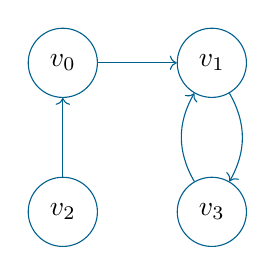
\begin{tikzpicture}
    \node[state,draw=goetheblau] (v0) {$v_0$};
    \node[state,draw=goetheblau] (v1) [right=1cm of v0] {$v_1$};
    \node[state,draw=goetheblau] (v2) [below=1cm of v0] {$v_2$};
    \node[state,draw=goetheblau] (v3) [right=1cm of v2] {$v_3$};

    \path[->]   (v0) edge[draw=goetheblau] (v1)
                (v2) edge[draw=goetheblau] (v0)
                (v1) edge[draw=goetheblau,bend left] (v3)
                (v3) edge[draw=goetheblau,bend left] (v1);
\end{tikzpicture} \\ 
$\qquad\,\,\,\mathcal{G}(4,4)$

\end{document}